\chapter{反向价差}
\section{反向跨期价差}
反向跨期价差是一个与“正常”跨期价差相反的头寸。在反向跨期价差中,交易者卖出 1 手长期看涨期权,并买入 1 手短期看涨期权。这个价差也可以用看跌期权来建立。两手看涨期权的行权价是相同的。

\section{反向比率价差(后式价差)}
一个更受欢迎的反向策略是反向看涨期权比率价差(reverse ratio call spread),它一般被称为后式价差(backspread)。在这种类型的价差里,\textbf{交易者按照一个行权价卖出 1 手看涨期权,然后按照更高的行权价买入若干手看涨期权}。

\begin{figure}[h]
    \centering
    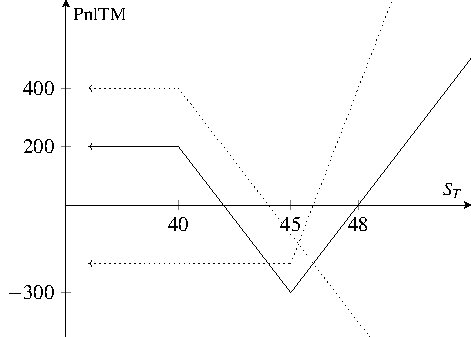
\includegraphics[width=0.7\textwidth]{IMG/Reverse ratio spread.pdf}
    \label{fig:Reverse ratio spread}
    \caption{XYZ 的售价是 43,7 月 40 看涨期权的售价是 4,卖出 1 手,7 月 45 看涨期权的售价是 1,买入 2 手。这个策略实际上是在一个熊市价差上加上一手看涨期权多头。}
\end{figure}

请注意,在这个价差中可以运用 delta 中性的概念,方法同用在看涨期权比率价差上基本一样。通过使用价差中期权的 delta,可以用数学方法计算出需买入和卖出的看涨期权的数量。

中性比率可以让交易者避免在开始时过于看空或者看多。例如,价差交易者如果只是为了方便而使用 2:1 而不是其他中性的比率,那么他就看得不够多。如果需要做点什么的话,价差交易者在建立这个价差时通常应当更侧重于看多,因为最大盈利是在上行方向。

在这类价差中,价差者必须对提前行权的可能性保持警觉,因为他卖出的是实值看涨期权。除了监控这种可能性之外,没有什么可以实施的后续防御行动,因为这个头寸的性质限制了它的风险。如果股票在期权到期之前大幅上涨,他可以将价差平仓,提走盈利。

这个策略代表了一种以少量的质押成本而能从股票的大幅运动中获利的合理方法。在贯彻这个策略的时候,一般而言,策略家应当寻找那些波动率较大的股票,因为他希望在看涨期权到期之前股价有尽可能大的运动。在\nameref{CH:Diagonalizing a Spread}里,我们将显示如果买入的看涨期权的存续期比卖出的看涨期权长时,这个策略有可能会变得更有吸引力